\section{Betrieb}
Für die Verwendung des Webinterface wird eine Netzwerkverbindung zum BeagleBone und ein Webbrowser\footnote{Das Webinterface verwendet \emph{JQuery} in der Version 2.1.1, aktuelle webbrowser sollten hier keine Probleme bereiten. Ansonsten kann die Homepage von JQuery konsultiert werden: \url{http://jquery.com/browser-support/}} mit aktiviertem JavaScript vorausgesetzt.


\subsection{Netzwerkverbindung herstellen}

\paragraph{Hinweis} Die Standardkonfiguration des BeagleBone sieht den Betrieb mit einem DHCP-Server vor. Sollte dies nicht gewünscht oder möglich sein, kann über die üblichen Wege eine statische IP eingestellt werden. Anleitungen hierzu findet man im Internet.\\

Steht ein DNS-Server zur Verfügung, kann der BeagleBone über seinen Hostname erreicht werden, standardmäßig \textit{boneserver}. Ansonsten finden Sie zunächst heraus, welche IP dem BeagleBone zugewiesen wurde. Hierfür kann entweder die Routing-Tabelle des DHCP-Servers konsultiert werden oder in der Kommandozeile via \emph{ip} die aktuelle Addresse der einzelnen Netzwerkadapter abgerufen werden \mbox{(Abb. \ref{fig:getBeagleBoneIP})}.

\begin{figure}[ht]
	\centering
	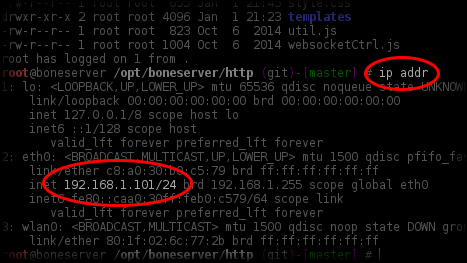
\includegraphics[width=0.7\textwidth]{images/getBeagleBoneIP.png}
	\caption{IP des BeagleBone abrufen}
	\label{fig:getBeagleBoneIP}
\end{figure}


\subsection{Webinterface aufrufen}
Das Webinterface kann einfach über DNS-Namen oder die IP im Webbrowser aufgerufen werden. Ist die Verbindung hergestellt, wird dies durch einen grünen Haken rechts in der Titelleiste angezeigt \mbox{(Abb. \ref{fig:mainWindowConnected})} und die Steuerelemente werden generiert.
Sollte die Verbindung einmal unterbrochen werden, wechselt dieser Haken in ein rotes Kreuz. In diesem Fall kann die Seite neu geladen werden, eventuelle Konfigurationen bleiben erhalten.

\paragraph{Passwortschutz} Um unbefugten Zugriff zu verhindern ist das Webinterface passwortgeschützt. Wenn Sie dieses Passwort änderen möchten, generieren Sie zunächst einen neuen Datensatz z. B. mit dem \href{http://jesin.tk/tools/htdigest-generator-tool/}{\textit{htdigest Generator Tool}}\footnote{ \url{http://jesin.tk/tools/htdigest-generator-tool/}} und tragen die Zugangsdaten in die Datei \textit{config/lighttpd/lighttpd.user} ein. Die Default Login-Daten sind \textbf{admin/AgG7KgW4}

\begin{figure}[ht] 
	\centering
	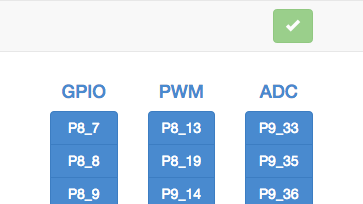
\includegraphics[]{images/mainWindowConnected.png}
	\caption{Webinterface verbunden}
	\label{fig:mainWindowConnected}
\end{figure}

\paragraph{Hinweis} Das Webinterface kann immer nur von einem Fenster aus aufgerufen werden. Es kann daher passieren, dass bei einem schnellen Fensterwechsel oder Neuladen der Seite die Verbindung nicht sofort hergestellt wird. In dem Fall einfach ein paar (Milli-)Sekunden warten, bis die Verbindung wieder frei ist.


\subsection{Bedienelemente}
Wie in \mbox{Abbildung \ref{fig:webinterface}} gezeigt hat die Weboberfläche des boneserver drei Anzeigegruppen:

\begin{itemize}
\item[\textbf{1}] \textbf{Verbindungsanzeige}\\
zeigt grün, wenn die Steuereinheit verbunden ist und rot, wenn die Verbindung unterbrochen ist (vgl. Abb. \ref{fig:mainWindowConnected}).
\item[\textbf{2}] \textbf{Bedienfelder} für digitale I/O, PWM und AIN\\
Hier findet die tatsächliche Bedienung der GPIO statt. Es gibt drei Sektionen jeweils für digitale I/O, PWM und AIN. Die Bedienung der verschiedenen Kacheln wird weiter unten beschrieben.
\item[\textbf{3}] \textbf{Anzeigenschalter} für die einzelnen Pins\\
Hier können einzelne Kacheln ein- bzw. ausgeblendet werden, um die Oberfläche übersichtlicher zu gestalten und an die Arbeitsumgebung anzupassen. Diese Funktion dient ausschließlich der Übersicht, eine ausgeblendete Kachel bleibt weiterhin aktiv und kann jederzeit wieder eingeblendet werden. Diese Einstellungen bleiben auch nach einem Neustart erhalten.
\end{itemize}

\begin{figure}[ht] 
	\centering
	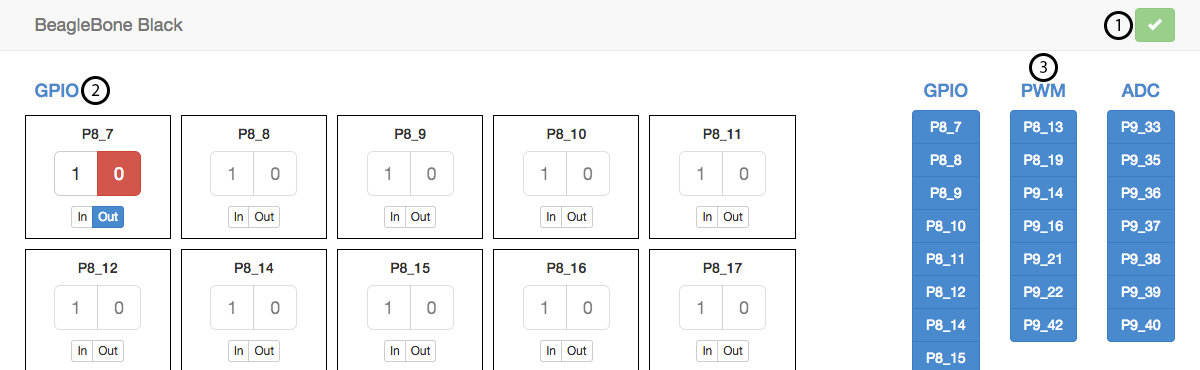
\includegraphics[width=1.0\textwidth]{images/controlElements.png}
	\caption{Weboberfläche}
	\label{fig:webinterface}
\end{figure}

\subsubsection{Digitale In- und Outputs}
Die Konfigurationskachel \mbox{(Abb. \ref{fig:mainWindowGPIODisabled})} für digitale I/O besteht aus zwei Schaltern: Betriebsrichtung und logic level.

\paragraph{Betriebsrichtung} Jeder digitale I/O kann entweder als Input oder als Output konfiguriert werden. Dazu kann über den Wahlschalter \textbf{In/Out} jederzeit das Gewüschte ausgewählt werden.

\paragraph{logic level} Wenn der GPIO als Output konfiguriert ist, kann hier mittels der beiden Schaltflächen, \textbf{1} und \textbf{0}, ein logisches high und ein logisches low eingestellt werden. Ist der GPIO als Input konfiguriert, ist diese Schaltfläche deaktiviert und zeigt stattdessen den Status der Leitung an. Die GPIO sind mit einem internen Pulldown-Widerstand beschaltet.

\begin{figure}[ht] 
	\centering
	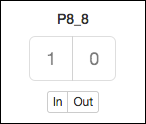
\includegraphics[]{images/mainWindowGPIODisabled.png}
	\caption{Deaktivierte GPIO-Kachel}
	\label{fig:mainWindowGPIODisabled}
\end{figure}


\subsubsection{Pulsbreitenmodulation (PWM)}
Mit Hilfe der PWM-Kacheln \mbox{(Abb. \ref{fig:mainWindowPWMDisabled})} werden die GPIO konfiguriert, über die eine Pulsbreitenmodulation möglich ist.\\

Der BeagleBone stellt insgesamt sieben PWM-Ausgänge mit insgesamt vier Timern zur Verfügung. Dabei teilen sich jeweils die Pinne P8\_13/19, P9\_14/16 und P9\_21/22 einen Timer. P9\_42 hat einen exklusiven Timer. Die Ausgänge mit einem gemeinsamen Timer haben dementsprechend immer dieselbe Frequenz und laufen absolut synchron.\\

Über die Buttons \textbf{Enable} und \textbf{Disable} kann der jeweilige Ausgang aktiviert bzw. deaktiviert werden. Wenn ein PWM-Ausgang deaktiviert wird, werden alle Einstellungen bezüglich Frequenz und Pulsbreite gelöscht!

\paragraph{Periodendauer} Über das Eingabefeld \textbf{Period} wird die Periodendauer in Nanosekunden (ns) eingestellt. Kleinster Wert ist hier 1 ns ($\hat{=}$ 1GHz) und der größte $10^9$ ns (= 1s $\hat{=}$ 1Hz).

\paragraph{Pulsbreite} Über das Eingabefeld \textbf{Duty} wird die Pulsbreite zwischen 0 und 1 eingestellt. Hier wird intern ebenfalls mit Nanosekunden gearbeitet, daher kann der tatsächliche Wert zusätzliche Nachkommastellen bekommen.

\begin{figure}[ht] 
	\centering
	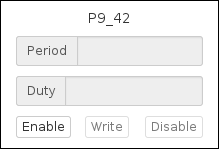
\includegraphics[]{images/mainWindowPWMDisabled.png}
	\caption{Deaktivierte PWM-Kachel}
	\label{fig:mainWindowPWMDisabled}
\end{figure}

Mit \textbf{Write} werden die Parameter abgesendet.

\paragraph{Hinweis} Der Linux Kernel arbeitet intern mit ganzen Nanosekunden, daher ist die Genauigkeit der Pulsbreite von der Höhe der Periodendauer anhängig.

\paragraph{Bug:} Wenn beide Ausgänge eines PWM-Generators aktiviert sind, lässt sich die Frequenz bei keinem der beiden ändern. Wenn bei einem der beiden PWMs die Frequenz zunächst geändert wurde, kann der zweite Ausgang nicht verwendet werden. Dies ist ein Problem der im Hintergrund verwendeten device tree overlays und wird in nachfolgenden Versionen der Bibliothek behoben.


\subsubsection{Analoge Inputs}
Mit diesen Kacheln \mbox{(Abb. \ref{fig:mainWindowADC})} werden die Analog/Digital-Converter gesteuert und die Eingangswerte in einem Echtzeitdiagramm angezeigt.\\

Mit den Tasten \textbf{Start} und \textbf{Stop} wird die Aufzeichnung gestartet bzw. gestoppt. Parallel zur Anzeige werden die Messdaten aufgezeichnet. Über \textbf{Download} können sie als CSV-Datei heruntergeladen werden.\\

Die Taste \textbf{Delete} löscht die zu diesem Eingang gespeicherte Messreihe um Speicherplatz frei zu machen.

\paragraph{\color{red} ACHTUNG} \textbf{\color{red} Laden sie Messreihen immer herunter, bevor Sie sie löschen, die Messdaten sind sonst unwiederbringlich verloren!}

\begin{figure}[ht] 
	\centering
	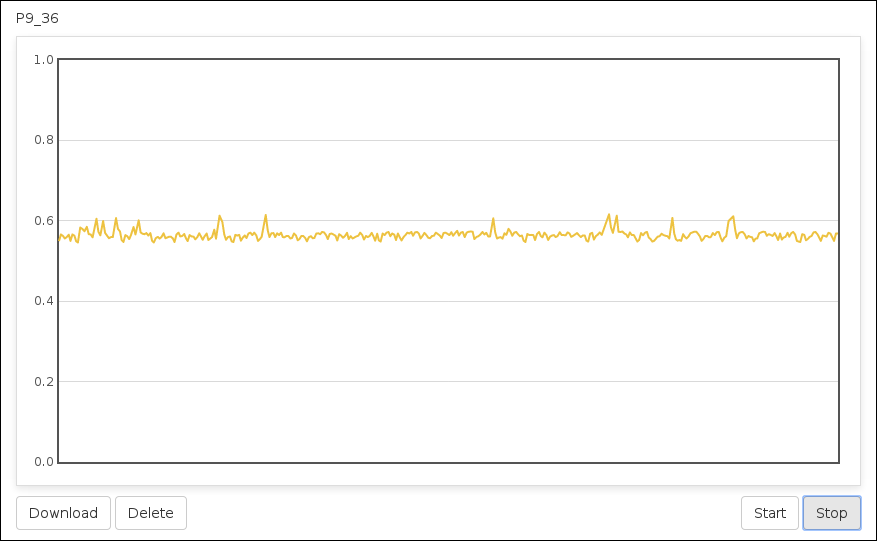
\includegraphics[width=0.9\textwidth]{images/mainWindowAIN.png}
	\caption{ADC-Kachel}
	\label{fig:mainWindowADC}
\end{figure}


\subsection{Erweiterte Einstellungen}
Zusätzlich gibt es die Möglichkeit, über die Datei \textit{settings.json} im root-Verzeichnis des boneserver weitere Einstellungen vorzunehmen. Ist keine solche Datei vorhanden, wird die mitgelieferte \textit{settings-default.json} verwendet. Die Parameter überschreiben die Default-Werte, es müssen daher nur abweichende Werte eingetragen werden.\\

Die Datei ist eine JSON\footnote{JavaScript Object Notation (JSON) ist in der RFC 7159 beschrieben}-Datei in der folgende Parameter eingestellt werden können:\\

\begin{longtabu} to \textwidth {X[1] X[3]}
    
  \textbf{host} & IP des WebSocket Servers\newline
  Dieser Wert sollte nicht verändert werden, da sonst der WebSocket Server möglicherweise nicht mehr über das Webinterface erreichbar ist.\newline
  \textit{default: localhost}\\
  \textbf{port} & Netzwerk-Port des WebSocket Servers\newline
  Dieser Wert sollte nicht verändert werden, da der WebSocket Server sonst nicht mehr über das Webinterface erreichbar ist.\newline
  \textit{default: 8081}\\
  \textbf{gpioSampleRate} & Abtastrate der digitalen Inputs in Millisekunden\newline
  Angegeben wird die Zeit zwischen den Abfragen. Dieser Wert kann erhöht werden um die System- und Netzwerklast zu verringern.\newline
  \textit{default: 100}\\
  \textbf{adcSampleRate} & Abtastrate der analogen Inputs in Millisekunden\newline
  Angegeben wird die Zeit zwischen den Abfragen. Dieser Wert kann erhöht werden, um die System- und Netzwerklast sowie um die Menge der erhobenen Messwerte zu verringern. Dies ermöglicht bei gleichem Speicherplatz längere Messreihen.\newline
  \textit{default: 10}\\
  \textbf{dataLocation} & Speicherpfad für die Messdaten der ADC\newline
  Hier kann ein alternativer Pfad zur Speicherung der Messdaten eintragen werden. Es können auch externe Speicherorte wie z. B. USB-Sticks, USB-Festplatten oder Netzlaufwerke verwendet werden.\newline
  \textit{default: ./data}
\end{longtabu}

\paragraph{Hinweis} Die Datei \textit{settings-default.json} sollte nicht verändert werden, da sonst nicht ohne weiteres ein Update durchgfeührt werden kann.
